\documentclass[11pt,spanish]{article}
\usepackage[utf8]{inputenc}
\usepackage{babel}
\usepackage{fullpage}
\usepackage{listings}
\usepackage{mathpazo}
\usepackage{enumitem}
\usepackage{courier}
\usepackage{xcolor}
\usepackage{textcomp}
\usepackage{amsmath}
\usepackage{amssymb}
\usepackage{tikz}
\usepackage{fancyhdr}
\usepackage{graphics}

\hyphenation{usua-rio usua-rios si-guen-te}

\newcommand{\titulo}{Certamen 2 tipo}
\newcommand{\cc}[1]{\hfil\texttt{#1}\hfil}
\newcommand{\pond}[1]{[{\small\textbf{#1\%}}]}

\pagestyle{fancy}
\lhead{%
  {\Large\bfseries Programación---\titulo} \\
  Nombre: \nombre\hfill
  Rol:    \rol
  \vspace{2ex}
}
\chead{}\rhead{}\lfoot{}\cfoot{}\rfoot{}
\renewcommand{\headrulewidth}{0pt}
\addtolength{\headheight}{7ex}
\headsep=4ex


\newcommand{\onelinerule}{\rule[2.3ex]{0pt}{0pt}}
\newcommand{\twolinerule}{\rule[6.2ex]{0pt}{0pt}}
\newcommand{\respuesta}{\framebox[\textwidth]{\twolinerule}}
\newcommand{\nombre}{%
  \begin{tikzpicture}[xscale=.4,yscale=.7]
    \draw (0, 0) rectangle (22, 1);
  \end{tikzpicture}%
}
%\newcommand{\rol}   {\framebox[0.3\textwidth]{\onelinerule}}
\newcommand{\rol}{%
  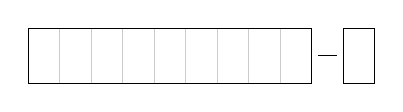
\begin{tikzpicture}[xscale=.4,yscale=.7]
    \draw[gray!40] ( 0, 0) grid      ( 9, 1);
    \draw          ( 0, 0) rectangle ( 9, 1);
    \draw          (10, 0) rectangle (11, 1);
    \draw (9 + .2, .5) -- (10 - .2, .5);
  \end{tikzpicture}%
}
\newcommand{\li}{\lstinline}
\providecommand{\pond}[1]{[{\small\textbf{#1\%}}]}

\lstdefinelanguage{py}{%
  classoffset=0,%
    morekeywords={%
      False,class,finally,is,return,None,continue,for,lambda,try,%
      True,def,from,nonlocal,while,and,del,global,not,with,print,%
      as,elif,if,or,yield,assert,else,import,pass,break,except,in,raise},%
    keywordstyle=\color{black!80}\bfseries,%
  classoffset=1,
    morekeywords={int,float,str,abs,len,raw_input,exit,range,min,max,%
      set,dict,tuple,list,bool,complex,round,sum,all,any,zip,map,filter,%
      sorted,reversed,dir,file,frozenset,open,%
      array,zeros,ones,arange,linspace,eye,diag,dot},
    keywordstyle=\color{black!50}\bfseries,%
  classoffset=0,%
  sensitive=true,%
  morecomment=[l]\#,%
  morestring=[b]',%
  morestring=[b]",%
  stringstyle=\em,%
}

\lstdefinelanguage{testcase}{%
  moredelim=[is][\bfseries]{`}{`},%
  backgroundcolor=\color{gray!20},%
}

\lstdefinelanguage{file}{%
  frame=single,%
}

\lstset{language=py}
\lstset{basicstyle=\ttfamily}
\lstset{columns=fixed}
\lstset{upquote=true}
\lstset{showstringspaces=false}
\lstset{rangeprefix=\#\ }
\lstset{includerangemarker=false}

\newlist{certamen}{enumerate}{1}
\setlist[certamen]{%
  label=\arabic*.,
  font=\LARGE\bfseries,%
  labelindent=-.5in,%
  leftmargin=0pt,%
  labelsep=1em%
}



\begin{document}

  \begin{enumerate}[font=\Large\bfseries]

    \item
      \pond{25}
      Indique qué es lo que imprimen los siguientes programas.

      \foreach \x in {1,2,...,8} {
        \noindent
        \begin{minipage}[b]{19.8em}
          \lstinputlisting{p\x.py}
          \framebox[18em]{\rule[6ex]{0pt}{0pt}}
          \vspace{0.7em}
        \end{minipage}
      }

    \newpage
    \item
      \pond{25}
      Los resultados de los campeonatos de fútbol desde 1990 en adelante
      están almacenados en los archivos \texttt{1990.txt}, \texttt{1991.txt},
      \ldots, \texttt{2009.txt} y \texttt{2010.txt}.

      Cada uno de los archivos
      tiene la información de todos los partidos de ese año,
      con el formato ilustrado
      en el siguiente ejemplo:

      \begin{minipage}{.5\textwidth}
        \begin{lstlisting}[language=file]
Huachipato-Puerto Montt:1-2
Fernandez Vial-O'Higgins:3-3
Rangers-Provincial Osorno:0-1
Coquimbo Unido-Deportes Temuco:2-0
        \end{lstlisting}
      \end{minipage}

      Escriba la función \li!estadisticas_equipo(nombre_equipo)!
      que reciba como parámetro el nombre de un equipo,
      y entregue como resultado
      una tupla con las cantidades de
      partidos ganados, empatados y perdidos
      por el equipo desde 1990:
      \begin{lstlisting}
>>> estadisticas_equipo('Santiago Morning')
(35, 24, 41)
      \end{lstlisting}

    \newpage
    \item
      \pond{25}
      La banda de rock Strip'n Split
      ha concluído su gira mundial.
      La información de cada uno de sus conciertos
      está almacenada en una lista
      en orden cronológico.

      \begin{minipage}[t]{.45\textwidth}
        Cada elemento de la lista
        es un diccionario con tres llaves:
        \li!'ciudad'!, \li!'publico'! y \li!'canciones'!.
        El valor asociado a \li!'publico'!
        es la cantidad de personas que asistió al concierto,
        y el asociado a \li!'canciones'!
        es la lista de las canciones que fueron tocadas
        en ese concierto.

        \begin{enumerate}
          \item
            Escriba una función llamada
            \li!cuantos_escucharon(c)!,
            que retorne la cantidad de personas
            que escucharon la canción \li!c!.
          \item
            Escriba una función llamada
            \li!mismo_concierto(c1, c2)!,
            que retorne \li!True! o \li!False!
            para indicar si las canciones \li!c1! y \li!c2!
            fueron tocadas alguna vez en el mismo concierto.
        \end{enumerate}
      \end{minipage}
      \hspace{2em}
      \begin{minipage}[t]{.55\textwidth}
        \small
        \lstinputlisting[linerange=CONCIERTOS-FIN\ CONCIERTOS]
           {pauta3-4.py}
      \end{minipage}

    \newpage
    \item
      \pond{25}
      (Este ejercicio es una continuación del anterior).

      El diccionario \li!ciudades!
      asocia a cada país
      una lista de las ciudades de ese país
      en las que tocó Strip'n Split:
      \lstinputlisting[linerange=CIUDADES-FIN\ CIUDADES]
         {pauta3-4.py}

      \begin{enumerate}
        \item Escriba la función \li!canciones_pais(p)!,
          que retorne el conjunto de las canciones
          que fueron tocadas en el país \li!p!.
        \item Escriba la función \li!contar_exitos(n)!,
          que retorne la cantidad de veces en que
          hubo dos conciertos consecutivos
          en el mismo país
          que tuvieron más de \li!n! espectadores.
      \end{enumerate}

  \end{enumerate}
\end{document}

